\documentclass[10pt]{beamer}
\usetheme[
%%% options passed to the outer theme
%    hidetitle,           % hide the (short) title in the sidebar
%    hideauthor,          % hide the (short) author in the sidebar
%    hideinstitute,       % hide the (short) institute in the bottom of the sidebar
%    shownavsym,          % show the navigation symbols
%    width=2cm,           % width of the sidebar (default is 2 cm)
%    hideothersubsections,% hide all subsections but the subsections in the current section
%    hideallsubsections,  % hide all subsections
    left               % right of left position of sidebar (default is right)
%%% options passed to the color theme
%    lightheaderbg,       % use a light header background
  ]{AAUsidebar}

% If you want to change the colors of the various elements in the theme, edit and uncomment the following lines
% Change the bar and sidebar colors:
%\setbeamercolor{AAUsidebar}{fg=red!20,bg=red}
%\setbeamercolor{sidebar}{bg=red!20}
% Change the color of the structural elements:
%\setbeamercolor{structure}{fg=red}
% Change the frame title text color:
%\setbeamercolor{frametitle}{fg=blue}
% Change the normal text color background:
%\setbeamercolor{normal text}{bg=gray!10}
% ... and you can of course change a lot more - see the beamer user manual.


\usepackage[utf8]{inputenc}
\usepackage[english]{babel}
\usepackage[T1]{fontenc}
% Or whatever. Note that the encoding and the font should match. If T1
% does not look nice, try deleting the line with the fontenc.
\usepackage{helvet}

% colored hyperlinks
\newcommand{\chref}[2]{%
  \href{#1}{{\usebeamercolor[bg]{AAUsidebar}#2}}%
}

\title[Adversarial-learning on shallow-neural-networks]% optional, use only with long paper titles
{Adversarial-learning on shallow-neural-networks}

% \subtitle{v.\ 1.4.0}  % could also be a conference name

\date{\today}

\author[Marc Moreaux] % optional, use only with lots of authors
{
  Marc Moreaux\\
  \href{mailto:mmorea13@student.aau.dk}{{\tt mmorea13@student.aau.dk}}
}
% - Give the names in the same order as they appear in the paper.
% - Use the \inst{?} command only if the authors have different
%   affiliation. See the beamer manual for an example

\institute[
%  {\includegraphics[scale=0.2]{aau_segl}}\\ %insert a company, department or university logo
  Dept.\ of Machine Learning\\
  Aalborg University\\
  Denmark
] % optional - is placed in the bottom of the sidebar on every slide
{% is placed on the title page
  Department of Machine Learning\\
  Aalborg University\\
  Denmark
  
  %there must be an empty line above this line - otherwise some unwanted space is added between the university and the country (I do not know why;( )
}


% specify a logo on the titlepage (you can specify additional logos an include them in 
% institute command below
\pgfdeclareimage[height=1.5cm]{titlepagelogo}{AAUgraphics/aau_logo_new} % placed on the title page
%\pgfdeclareimage[height=1.5cm]{titlepagelogo2}{graphics/aau_logo_new} % placed on the title page
\titlegraphic{% is placed on the bottom of the title page
  \pgfuseimage{titlepagelogo}
%  \hspace{1cm}\pgfuseimage{titlepagelogo2}
}


\begin{document}
% the titlepage
{\aauwavesbg%
\begin{frame}[plain,noframenumbering] % the plain option removes the sidebar and header from the title page
  \titlepage
\end{frame}}
%%%%%%%%%%%%%%%%

% TOC
\begin{frame}{Agenda}{}
\tableofcontents
\end{frame}


%###############################
%###  INTRO
%###############################
\section{Introduction}
\begin{frame}{Introduction}{}
  \begin{itemize}
    \item<1-> Why are shallow-feed-forward-neural-networks not resistant to adversarial-samples ?
    \item<1-> Can adversarial-learning improve shallow-feed-forward-neural-networks' learning, and why ?
    \item<2-> Continue the work made by Ian J. Goodfellow, Jonathon Shlens and Christian Szegedy in "Explaining and Harnessing Adversarial Examples".    
  \end{itemize}
\end{frame}


\subsection{Explaining and harnessing adversarial examples}
\begin{frame}{Introduction}{Explaining and harnessing adversarial examples}
  \begin{block}{Explaining and harnessing adversarial examples}
    \begin{itemize}
      \item<1-> Neural-networks consistently mis-classify adversarial examples.
      \item<2-> Caused by linear nature of the network.
      \item<3-> Can be overcome with adversarial-learning.
    \end{itemize}
  \end{block}
\end{frame}



%###############################
%###  BACKGROUND
%###############################
\section{Background}
\subsection{Neural-networks}
\begin{frame}{Background}{Neural-networks}
  \begin{block}{Neurons}
    Artificial representation of a biological Neuron.
    \pause
    \begin{figure}
      \centering
      \def\layersep{1.5cm}
      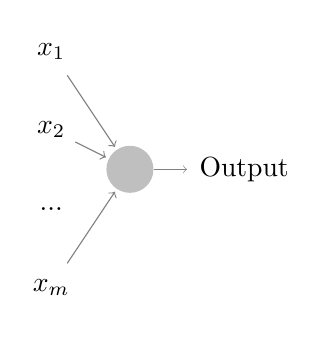
\begin{tikzpicture}[shorten >=1pt,->,draw=black!50, node distance=\layersep]
        \tikzstyle{tata}=[,minimum size=17pt,inner sep=0pt]
          \tikzstyle{neuron}=[circle,fill=black!25,minimum size=17pt,inner sep=0pt]
          \tikzstyle{output neuron}=[neuron, fill=red!50];

          % Input neurons
          \node[tata] (x1) at (0,-1 cm) {$x_1$};
          \node[tata] (x2) at (0,-2 cm) {$x_2$};
          \node[tata] (x3) at (0,-3 cm) {...};
          \node[tata] (x4) at (0,-4 cm) {$x_m$};
          
          % Draw the output layer node
          \node[neuron,pin={[pin edge={->}]right:Output}] (O) at (\layersep,-2.5) {};

          % Connect every node in the hidden layer with the output layer
          \path (x1) edge (O);
          \path (x2) edge (O);
          \path (x4) edge (O);

      \end{tikzpicture}
      \caption{Model of an artificial neuron}
      \label{fig:perceptron}
    \end{figure}
  \end{block}
\end{frame}

\begin{frame}{Background}{Neural-networks}
  \begin{block}{Neural-network}
    Artificial network of neurons.
    \pause
    \begin{figure}
      \centering
      \def\layersep{1.5cm}
      \resizebox{.5\textwidth}{!}{
        \begin{tikzpicture}[shorten >=1pt,->,draw=black!50, node distance=\layersep]
            \tikzstyle{every pin edge}=[<-,shorten <=1pt]
            \tikzstyle{neuron}=[circle,fill=black!25,minimum size=17pt,inner sep=0pt]
            \tikzstyle{annot} = [text width=4em, text centered]


            %%%%%%%%%%%%%%%%%%%%%%%%%%%%%%%%%%%%%%%%%%%% 
            %%% DRAW THE NODES
            %%%%%%%%%%%%%%%%%%%%%%%%%%%%%%%%%%%%%%%%%%%%
            \foreach \name / \y in {1,...,4}
                \node[] (I-\name) at (0,-\y) {$x_{i\y}$};

            \foreach \name / \y in {1,...,5}
                \path[yshift=0.5cm] node[neuron] (H1-\name) at (\layersep,-\y cm) {};

          \foreach \name / \y in {1,...,7}
                \path[yshift=1.5cm] node[neuron] (H2-\name) at (\layersep*2,-\y cm) {};   

              
            \node[neuron,pin={[pin edge={->}]right:$p_{i1}$}, right of=H2-3] (O-1) {};
            \node[neuron,pin={[pin edge={->}]right:$p_{i2}$}, right of=H2-5] (O-2) {};

            %%%%%%%%%%%%%%%%%%%%%%%%%%%%%%%%%%%%%%%%%%%% 
            %%% DRAW THE PATHS
            %%%%%%%%%%%%%%%%%%%%%%%%%%%%%%%%%%%%%%%%%%%%
            \foreach \source in {1,...,4}
                \foreach \dest in {1,...,5}
                    \path (I-\source) edge (H1-\dest);

            \foreach \source in {1,...,5}
                \foreach \dest in {1,...,7}
                    \path (H1-\source) edge (H2-\dest);

            \foreach \source in {1,...,7}
              \foreach \dest in {1,...,2}
                  \path (H2-\source) edge (O-\dest);

            % Annotate the layers
            \node[annot,above of=H2-1, node distance=1cm] (hl) {Hidden layer 2};
            \node[annot,left of=hl] (hl1) {Hidden layer 1};
            \node[annot,left of=hl1] {Input layer};
            \node[annot,right of=hl] {Output layer};
        \end{tikzpicture}
      }
      \caption{Feed-forward neural-network with two hidden layers}
      \label{fig:feed_forward}
    \end{figure}
  \end{block}
\end{frame}

\subsection{Adversarial-learning}
\begin{frame}{Background}{Adversarial-learning}
  \begin{block}{Adversarial-example}
    Worst case example build from an original sample and the knowledge we have from the model.
  \end{block}
  \pause
  $$ \tilde{\boldsymbol{x}} = \boldsymbol{x} + \eta $$
  $$ \eta = \epsilon_{\text{adv}} \times \text{sign}(\nabla_x \text{Cost}(\boldsymbol{W},\boldsymbol{x},\boldsymbol{y})) $$
  \vskip 1cm
  \pause
  \begin{block}{Adversarial-learning}
    Training based on adversarial-samples
  \end{block}
\end{frame}


\subsection{Datasets}
\begin{frame}{Background}{Datasets}
  \begin{block}{MNIST}
    70k images belonging in the 10 digits. Each sample is 28*28 gray-scale pixel with value $[0,1]$.
   \begin{figure}
      \centering
      \includegraphics[width=0.6\textwidth]{/home/marc/git/MI10_adversarial_training/training_test/MLP3/mem/bar_MNIST_orig.png}
    \end{figure}
  \end{block}
  \pause
  \vskip -.5cm

  \begin{block}{CIFAR10}
    60k images belonging in 10 classes. Each sample is made 32*32 gray-scale pixel with value $[0,1]$.
    \begin{figure}
      \centering
      \includegraphics[width=0.6\textwidth]{/home/marc/git/MI10_adversarial_training/training_test/MLP3/mem/bar_orig_CIFAR.png}
    \end{figure}
  \end{block}
  \pause
  \vskip -.5cm

  \begin{block}{COVType}
    581k inputs belonging in 7 classes. Classify the predominant kind of tree cover from strictly cartographic variables.
  \end{block}
  
\end{frame}

%###############################
%###  EXPERIENCES
%###############################
\section{Experiences}

\subsection{MNIST playing with neurons quantities}
\begin{frame}{Experiences}{MNIST playing with neurons quantities}
  \pause
  \begin{figure}
    \centering
    \includegraphics[width=0.7\textwidth]{/home/marc/git/MI10_adversarial_training/training_test/MLP3/mem/bar_neuron_impact.png}
    \caption{Comparing the amount of neurons' impact on non-adversarial and adversarial models. Every pair represent a non-adversarial-learning and an adversarial-learning trained with a certain amount of hidden neurons.}
    \label{fig:mnist_neurons}
  \end{figure}
\end{frame}

\subsection{MNIST playing with adversarial epsilon}
\begin{frame}{Experiences}{MNIST playing with adversarial epsilon}
  \pause
  \begin{figure}
    \centering
    \includegraphics[width=0.7\textwidth]{/home/marc/git/MI10_adversarial_training/training_test/MLP3/mem/bar_eps_imapct.png}
    \caption{Evaluate non-adversarial and adversarial models of 800 hidden neurons.}
    \label{fig:mnist_adv_eps}
  \end{figure}
\end{frame}

\subsection{MNIST test on noisy dataset}
\begin{frame}{Experiences}{MNIST test on noisy dataset}
  \pause
  \begin{figure}
    \centering
    \includegraphics[width=0.4\textwidth]{/home/marc/git/MI10_adversarial_training/training_test/MLP3/mem/bar_testset_impact_adv.png}
    \includegraphics[width=0.4\textwidth]{/home/marc/git/MI10_adversarial_training/training_test/MLP3/mem/bar_testset_impact_norm.png}
    \caption{Evaluate non-adversarial (dashed line) and adversarial models (plain line) of 800 hidden neurons on modified test-sets. On the left, we try the two models on an adversarial test-dataset. The horizontal axis represents the epsilon values used to modified the test-set. On the right, we try the two models on an normal-distribution-modified test-dataset with different standard deviations.}
    \label{fig:mnist_adv_noisy_ds}
  \end{figure}
\end{frame}

\begin{frame}{Experiences}{MNIST test on noisy dataset}
  \pause
  \begin{figure}
    \centering
    \includegraphics[width=0.7\textwidth]{/home/marc/git/MI10_adversarial_training/training_test/MLP3/mem/bar_noisy_ts_adv.png}\\
    \includegraphics[width=0.7\textwidth]{/home/marc/git/MI10_adversarial_training/training_test/MLP3/mem/bar_noisy_ts_norm.png}
    \caption{Extract of the test-set with the same image with different noises. On the top, you see the adversarial noised sample with $\epsilon_{\text{ads}} = [.0, .1, .2, .3]$. On the bottom you see the uniform noised sample with, from left to right the standard deviation taking values: $\epsilon_{\text{noise}} = [.0, .1, .2, .3]$}
    \label{fig:mnist_adv_noisy_ds_img}
  \end{figure}
\end{frame}

\subsection{MNIST compare with other traning method}
\begin{frame}{Experiences}{MNIST compare with other traning method}
  \pause
  \begin{figure}
    \centering
    \includegraphics[width=0.4\textwidth]{/home/marc/git/MI10_adversarial_training/training_test/MLP3/mem/bar_testset_impact_2_adv.png}
    \includegraphics[width=0.4\textwidth]{/home/marc/git/MI10_adversarial_training/training_test/MLP3/mem/bar_testset_impact_2_norm.png}
    \caption{Evaluate normal-distribution-based model versus the casual and adversarial models of 800 hidden neurons on noisy test-sets and adversarial datasets.}
    \label{fig:mnist_noisy_learn}
  \end{figure}
\end{frame}

\subsection{MNIST visualize weights}
\begin{frame}{Experiences}{MNIST visualize weights}
  \pause
  \begin{figure}
    \centering
    \includegraphics[width=0.4\textwidth]{/home/marc/git/MI10_adversarial_training/training_test/MLP3/mem/bar_weight_class_800.png}
    \caption{Attempt at visualizing classes pattern on casual-model (top) and adversarial-model (bottom) of 800 neurons (left) and 2000 neurons (right).}
    \label{fig:mnist_weight_class}
  \end{figure}
\end{frame}

\subsection{CIFAR10 adversarial traning}
\begin{frame}{Experiences}{CIFAR10 adversarial traning}
  \pause
  \begin{figure}
    \centering
    \includegraphics[width=0.4\textwidth]{/home/marc/git/MI10_adversarial_training/training_test/MLP3/mem/bar_testset_impact_adv_CIFAR.png}
    \includegraphics[width=0.4\textwidth]{/home/marc/git/MI10_adversarial_training/training_test/MLP3/mem/bar_testset_impact_norm_CIFAR.png}
    \caption{Evaluate non-adversarial (dashed line) and adversarial models (plain line) of 2500 hidden neurons on modified test-sets. On the left, we try the two models on an adversarial test-dataset. The horizontal axis represents the epsilon values used to modified the test-set. On the right, we try the two models on an normal-distribution-modified test-dataset with different standard deviations.}
    \label{fig:cifar_noisy_test}
  \end{figure}
\end{frame}

\subsection{COVType adversarial traning}
\begin{frame}{Experiences}{COVType adversarial traning}
  \pause
  \begin{table}[ht]
    \centering
    \begin{tabular}{c||c|c|c|c|c}
      hidden neurons & 60 & 80 & 100 & 120 & 150 \\
      \hline
      non-adversarial & $.5103$ & $.5107$ & $.5116$ & $.5108$ & $.5108$ \\
      adversarial     & $.5106$ & $.5111$ & $.5103$ & $.5106$ & $.5116$ \\
    \end{tabular}
    \caption{Accuracy of adversarial and non-adversarial models with different amount of hidden neurons on the Covertype dataset.}
    \label{tab:cov_acc}
  \end{table}
\end{frame}



{\aauwavesbg
\begin{frame}[plain,noframenumbering]
  \finalpage{Thank you for your attention }
\end{frame}}
%%%%%%%%%%%%%%%%

\end{document}
